\documentclass[12pt,a4paper]{article}
\usepackage{amsmath}
\usepackage{amsfonts}
\usepackage{amssymb}
\usepackage{accsupp}
\usepackage[ruled,vlined]{algorithm2e}
\usepackage{float}
\usepackage{subfig}
\usepackage{graphicx}


\usepackage{fancyhdr}
\pagestyle{fancy}
\fancyhf{}
\fancyhf[rh]{\thepage}

\begin{document}
\title{A Brief Overview of Byte Digraphs}
\author{James Oswald}

\maketitle

\section{Introduction}
The work of Sergey Bratus and Greg Conti in Digraph data visualization for binary sequences is under-explored mathematically and is largely unformalized. This has lead to it being largely forgotten outside of a few open source cyber-security projects. I hope to introduce digraphs and provide a few formal definitions for working with them. 

\section{Binary Digraphs}
\subsection{Formalization of The Core Concept}
Bratus et al. posit that even binary data we expect to be unstructured or random is in fact structured in a way we wouldn't expect. The key idea is that each byte $b_k$ in a byte sequence $B$ of length $n$ has an implicit binary relation with the byte following it, $b_{k+1}$. We can define this relation in set builder notation as: 
\[
R = \{(b_k, b_{k+1})|b_k\in B \wedge k<n\} \tag{2.1} \label{Rel}
\]
We can then graph this relation to image coined a "Digraph", which is simply a plot of $R$ in $\mathbb{N}^2$ which gives rise to noticeable artifacts that can be used to classify data. Alternatively, I propose a digraph can be represented using a binary matrix $M_{256\times256}$  who's entries are set according to: 
\[
M_{ij} = 
\left\{
\begin{array}{ll}
1 & \mbox{if }(b_i, b_j)\in B \\
0 & \mbox{if }(b_i, b_j)\notin B
\end{array}
\right.
\tag{2.2} \label{Mat}
\]
Since these digraphs are represented using a binary matrix, I will be referring to them as "binary digraphs"

\pagebreak
\subsection{Formalizing a Binary Digraph Generator Algorithm}
The Digraph Algorithm I pose here uses the process of constructing the binary matrix described by \eqref{Mat}.
\begin{algorithm}
\DontPrintSemicolon
\SetKwInOut{Input}{input}
\SetKwInOut{Output}{output}
\Input{A Binary sequence $B = \{b_0, b_1, ..., b_n\}$}
\Output{A Binary Digraph in the form of the binary matrix $M_{256\times256}$}
\BlankLine
$M = \textbf{0}_{256\times256}$\;
\For{$i = 0$ to $n - 1$}{
	$M_{b_{i}b_{i+1}} = 1$\;
}
\caption{Generate Binary Digraph}
\label{bdgA}
\end{algorithm}

It is trivially proved that this algorithm is $\mathcal{O}(n)$ 

\subsection{Visualizing Binary Digraphs}
By taking our binary matrix $M$ and converting it to a bitmap such that 0 is black and 1 is red, We can instantly see shocking artifacts that allow us to distinguish the type of data we're looking at.

For these first three binary digraphs, I have converted three full books into byte strings and applied algorithm 1 generating the following bitmaps:

\begin{figure}[!h]
    \centering
    \subfloat[Digraph of The Republic]{
		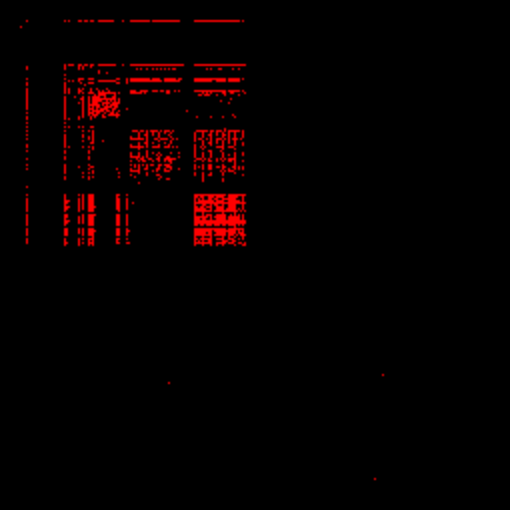
\includegraphics[scale=0.25]{images/TheRepublic.png} 
    }
    \subfloat[Digraph of Alice in Wonderland]{
		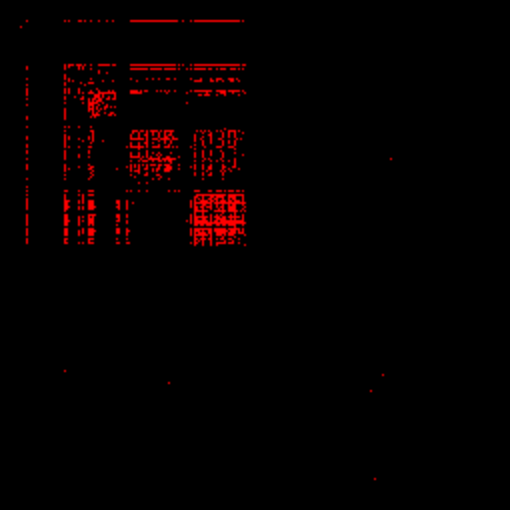
\includegraphics[scale=0.25]{images/AliceInWonderLand.png}
    }
    \subfloat[Digraph of The Bible]{
		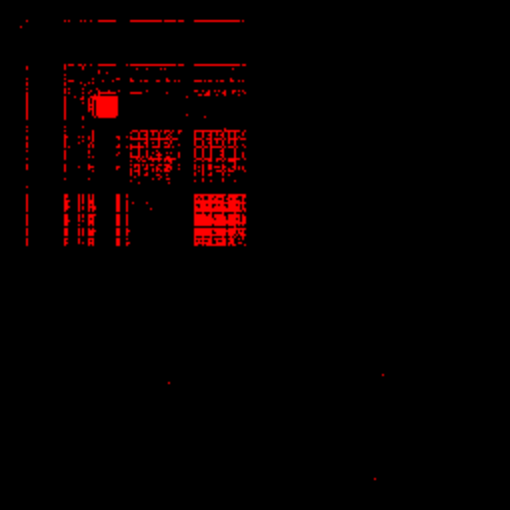
\includegraphics[scale=0.25]{images/TheBible.png}
    }
    \caption{Book Digraphs}
    \label{ref_label_overall}
\end{figure}

\pagebreak
The obvious question that comes to mind when viewing these digraphs is: Why do all 3 of these completely different books have very similar digraphs? The answer lies in ASCII encoding, these pasterns are the result of the relationship between subsequent ASCII characters. This can be broken down if we zoom in and begin classifying regions based on the sequence of bytes (or in our case, characters) that gave rise to them. 
\linebreak
\begin{minipage}{0.6\textwidth}
	\begin{figure}[H]
		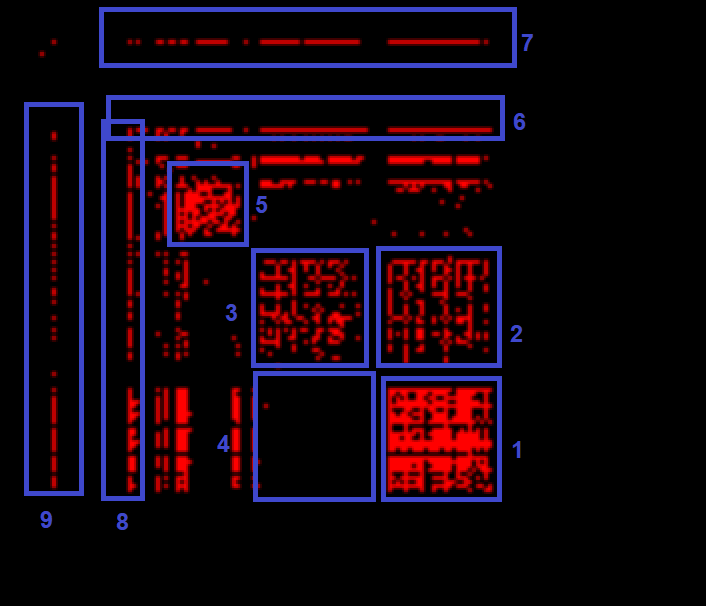
\includegraphics[scale=0.45]{images/RepublicZoom.png} 
		\caption{Digraph of Plato's The Republic}
	\end{figure}
\end{minipage} \hfill
\begin{minipage}{0.45\textwidth}
	\begin{itemize}
		\item 1)(lowercase, lowercase)
		\item 2)(uppercase, lowercase)
		\item 3)(uppercase, uppercase)
		\item 4)(lowercase, uppercase)
		\item 5)(digit, digit)
		\item 6)(character, space)
		\item 7)(character, new Line)
		\item 8)(space, character)
		\item 9)(new Line, character)
	\end{itemize}
\end{minipage}
\linebreak\linebreak\linebreak
Notice that this produces results that are intuitively easy to understand as well, we would expect an English book to be primarily composed of mostly lowercase letters followed by lowercase letters, while we would expect no lowercase letters followed by uppercase letters, which is exactly what we see in section 4. 

\pagebreak
\begin{samepage}
\subsection{Limitations of Binary Digraphs}
In the last section we looked at Digraphs of text data, In this section we'll explore Digraphs of more types of data and see the limitations of binary digraphs. 
\begin{figure}[!h]
    \centering
    \subfloat[Digraph of a .exe (Machine Code Data)]{
		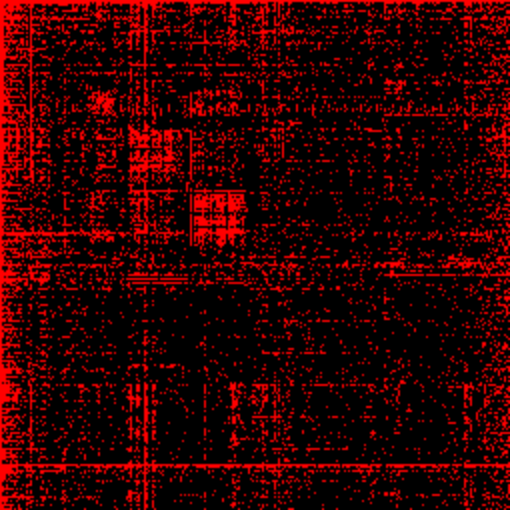
\includegraphics[scale=0.35]{images/exe.png} 
		\label{Sp1}
    }
    \subfloat[Digraph of a .wav (Raw Audio Data)]{
		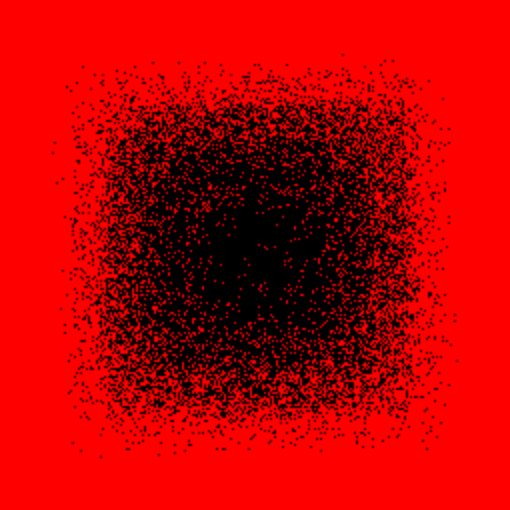
\includegraphics[scale=0.35]{images/wav.png}
		\label{Sp2}
    }
    \caption{Sparse}
\end{figure}
\begin{figure}[!h]
    \centering
    \subfloat[Digraph of a .gif (Compressed Image Data)]{
		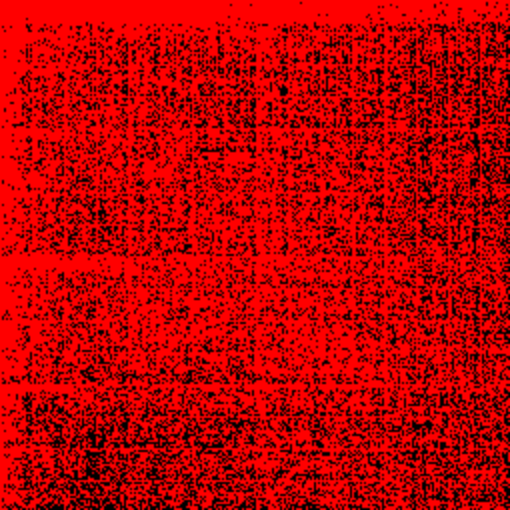
\includegraphics[scale=0.35]{images/gif.png}
		\label{De1}
    }
    \subfloat[Digraph of a .webm (Compressed Video Data)]{
		
\includegraphics[scale=0.35]{images/webm.png}
		\label{De2}
    }
    \caption{Dense}
\end{figure}
\end{samepage}
\pagebreak

These binary digraphs give us lots of insight into the intrinsic structure of this data and let us analyze entire files from just these snapshots. An analysis of \ref{Sp1} shows characteristic striping which is present in digraphs of all kinds of machine code, we also see the ascii regions are extra dense, so we can infer that there are a lot of embedded strings within this exe file. An analysis of \ref{Sp2} reveals yet another striking pattern produced by the digraph, characteristic of uncompressed audio data. 

\ref{De1} and \ref{De2} are where the usefulness of binary digraphs begin to run out, while \ref{De1} still shows a semblance of structure characteristic to compressed image data, the Digraph in \ref{De2} is so dense that it provides us with no meaningful structure, only letting us know that the data is compressed. 

\section{Positive Discrete Digraphs}
\subsection{Surpassing Binary Digraphs with Positive Discrete Digraphs}
In order to remedy this issue, I have developed what I will refer to as positive discrete digraphs to preserve more information and hence allow for better visualization. Rather then entires of the matrix $M$ being restricted to the set $\{0, 1\}$ as was the case with binary digraphs, I restrict entries to the non-negative integers $\mathbb{Z}^{\ast}$. The entries in the new matrix now represent the "count" of a sequential pair in $B$. In other words $M_{ij}$ is now the number of times $(b_i, b_j)$ appears in $R$
\subsection{Positive Discrete Digraph Generator Algorithm}
The algorithm is fundamentally the same as the Digraph Algorithm  but we add one to the entry instead of setting it to one. 
\begin{algorithm}
\DontPrintSemicolon
\SetKwInOut{Input}{input}
\SetKwInOut{Output}{output}
\Input{A Binary sequence $B = \{b_0, b_1, ..., b_n\}$}
\Output{A Positive Discrete Digraph in the form of the matrix $M_{256\times256}$}
\BlankLine
$M = \textbf{0}_{256\times256}$\;
\For{$i = 0$ to $n - 1$}{
	$M_{b_{i}b_{i+1}} = M_{b_{i}b_{i+1}} + 1$\;
}
\caption{Generate Positive Discrete Digraph Digraph}
\end{algorithm}

It is trivially proved that this algorithm is $\mathcal{O}(n)$ 
\subsection{Visualizing Positive Discrete Digraphs}
\subsubsection{Post-Processing Algorithm}
Unfortunately, coloring a bitmap solely from the positive discrete digraph alone produces lack luster results and doesn't show off the full potential of the information stored within the the positive discrete digraph. To get around this, I apply a post-processing algorithm that uses the median of the vectorization of the positive discrete digraph to help "center" the data for better viability. I then use this "centered" data to generate a bitmap, MAP, which for the purpose of this algorithm, will be a 256 by 256 matrix of 3-tuples representing RGB color channels who's values are integers between 0 and 255. 

\begin{algorithm}
\DontPrintSemicolon
\SetKwInOut{Input}{input}
\SetKwInOut{Output}{output}
\Input{A Positive Discrete Digraph $M$ in the form of a 256 by 256 matrix}
\Output{A Bitmap MAP in the form of a matrix of 3-tuples representing RGB Color channels}
\BlankLine
Med $=$ Median(Vectorize($M$))\;
MAP = $\begin{bmatrix}(0,0,0)_{0,0} & \ldots & (0,0,0)_{255,0}\\\vdots &\ddots&\vdots\\(0,0,0)_{0,255} & \ldots & (0,0,0)_{255,255}\\\end{bmatrix}$\;
\For{$i = 0$ to $255$}{
	\For{$j = 0$ to $255$}{
		MAP$_{ij}=(M_{ij}-$Med$+127, 0, {-M}_{ij}+$Med$ + 127)$
	}
}
\caption{Positive Discrete Digraph Post-Processing}
\end{algorithm}
\subsubsection{Visual PDD Results}
(See Next Page)
\pagebreak
\begin{figure}[H]
    \centering
    \subfloat[PDD of the Bible]{
		\includegraphics[scale=0.33]{images/biblePDD.png} 
		\label{PDD1}
    }
    \subfloat[PDD of a .wav (Raw Audio Data)]{
		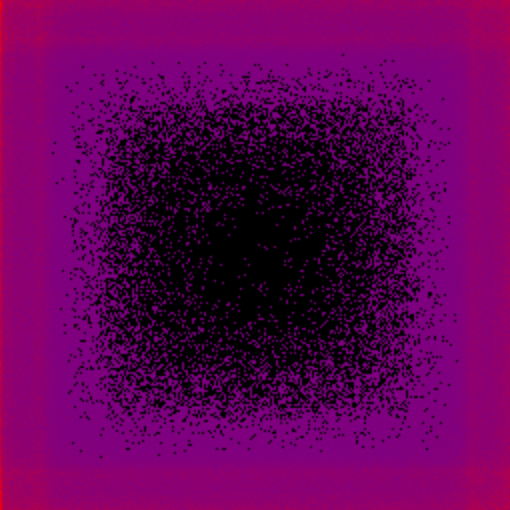
\includegraphics[scale=0.33]{images/wavPDD.png}
		\label{PDD2}
    }
    
    \subfloat[PDD of a .exe (Machine Code Data)]{
		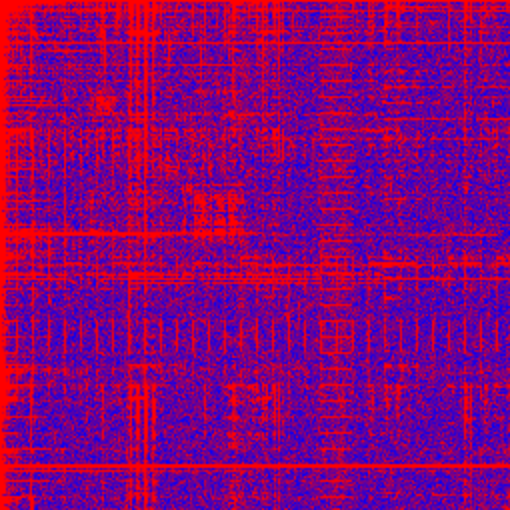
\includegraphics[scale=0.33]{images/exePPD.png} 
		\label{PDD3}
    }
    \subfloat[PDD of a .zip (Compressed Data)]{
		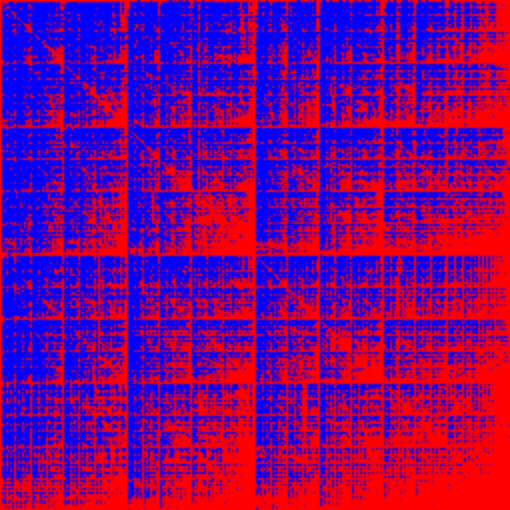
\includegraphics[scale=0.33]{images/zip.png}
		\label{PDD4}
    }
    
    \subfloat[Digraph of a .bmp (Raw Image Data)]{
		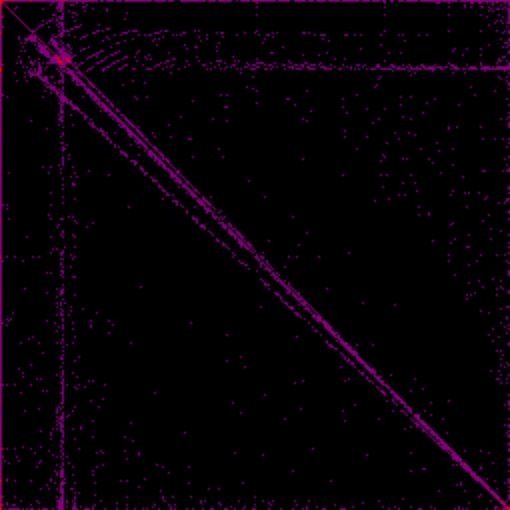
\includegraphics[scale=0.33]{images/bmp.png}
		\label{PDD5}
    }
    \subfloat[Digraph of an .msi (windows installer)]{
		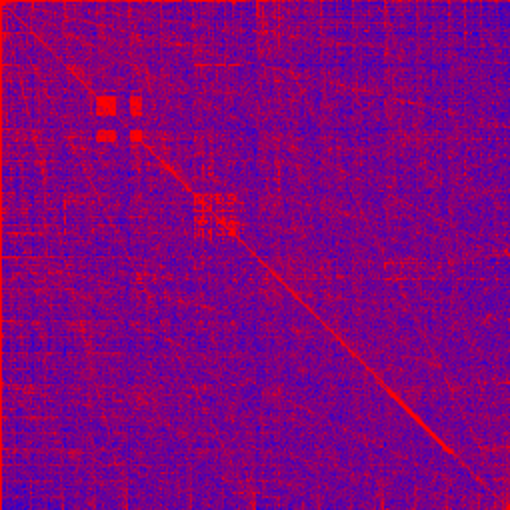
\includegraphics[scale=0.33]{images/msi.png} 
		\label{PDD6}
    } 
	\caption{"Positive Discrete Digraph Visual Results"}
\end{figure}
\pagebreak

\subsubsection{Analysis of PDD Results}
Under the new light provided by positive discrete digraphs with post processing, we can see structure 
that was previously hidden. In fact, \ref{PDD3}, \ref{PDD4}, \ref{PDD6}, would all look the same when seen from a binary digraph bitmap, but using positive discrete digraphs we can see that all 3 actually have wildly different structures. 

Upon re-analyzing \ref{PDD1} we see exactly what we expected from the ascii data, The red coloration in the (lowercase, lowercase) region tells us that all of these sequences occurred well above the median, while other regions were closer to the median and thus appear purple.

Re-analyzing \ref{PDD2} we see a bit more structure appear around the edges, however its easy to forget that the lack of real definition in the form of reds and blues is a sign that all central sequences appear at the same relative frequency, which itself is an important structural insight gained through  a PDD bitmap.

\ref{PDD3} is a large x86 machine code file (a windows .exe) that contains the telltale machine code striations discussed in section 2.4. Its also good to note that none of these would have been visible on a binary digraph and this would have looked identical to the .gif file in image \ref{De2}.

\ref{PDD4} is a 300MB zip file, it makes sense that every spot would be filled with that many bytes, but it has a surprising structure that much like \ref{PDD3} would not have been seen without the PDD bitmap.

\ref{PDD5} is a bitmap file storing raw image data, the diagonal stripe in the center is indicative of subsequent bytes having a similar value.

\ref{PDD6} is perhaps the most interesting digraph yet. It's a Windows Installer file, and it looks like a combination of \ref{PDD1}, \ref{PDD3}, \ref{PDD4}, \ref{PDD5}, and that's because it is. We can infer from the digraph that it contains alot of bitmaps from the red streak down the center, a lot of ascii data from the squares in the top right, and machine code from the heavy parallel striations. 



\end{document}